\begin{figure}[h]
\centering
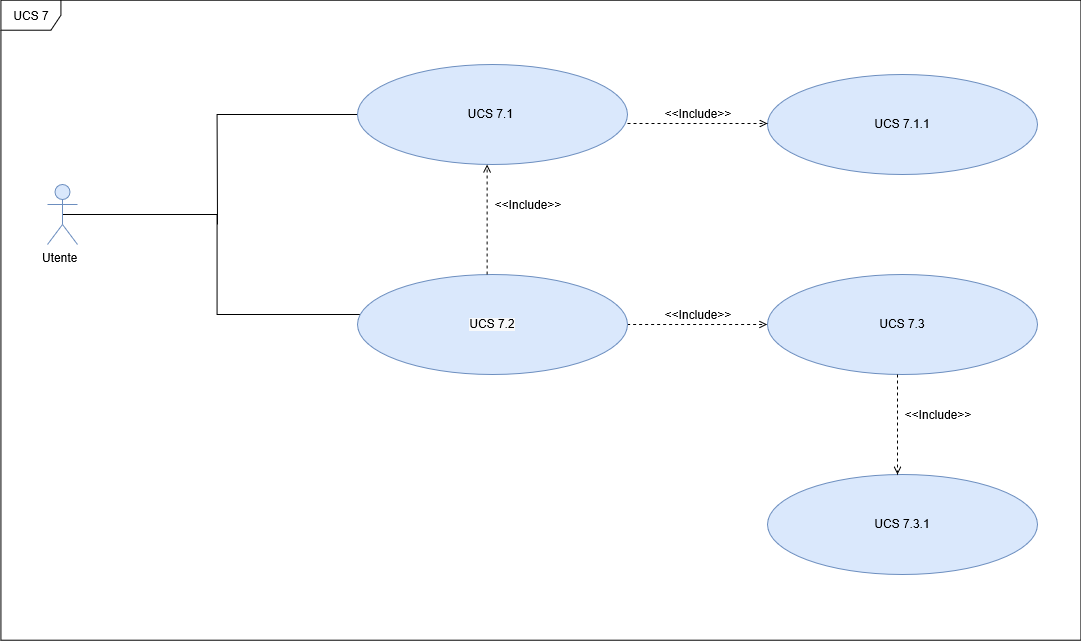
\includegraphics[scale=0.3]{sezioni/UseCase/Immagini/UCS7.png}%location immagine.   immagini/immagine.png
\caption{UCS 7 - Visualizzazione della lista degli accessi di un utente riconosciuto}
\label{logo}
\end{figure}

% UC... specificare App o Server -> UCA / UCS
\section{UCS 7}%kite level
\begin{itemize}
\item \textbf{Nome:} Visualizzazione della lista degli accessi di un utente riconosciuto di un'organizzazione
\item \textbf{Attori primari:} Amministratore visualizzatore
\item \textbf{Precondizione:} L’amministratore deve essere autenticato presso il sistema
\item \textbf{Postcondizione:} L’amministratore avrà visualizzato una lista degli accessi di un utente riconosciuto dell'organizzazione scelta
\item \textbf{Scenario principale:} L’amministratore, dopo aver selezionato l'organizzazione, accede alla funzionalità di visualizzazione della lista degli accessi di un utente riconosciuto e, dopo averlo selezionato, potrà visualizzare la sua lista degli accessi
\item \textbf{Flusso di eventi:} 
\begin{enumerate}
	\item UCS 3 l'amministratore ha selezionato l'organizzazione;
	\item l'amministrazione deve selezionare la funzionalità di visualizzazione della lista degli accessi
\end{enumerate}
\item \textbf{Estensioni:} Visualizzazione di un messaggio che informa l’indisponibilità del server [?????]
\item \textbf{Inclusioni:}
\begin{enumerate}
	\item UCS 3 l'amministratore ha selezionato l'organizzazione;
\end{enumerate}
\end{itemize}

\subsection{UC 7.1}%sea level
\begin{itemize}
\item \textbf{Nome:} Visualizzazione degli accessi di un'utente riconosciuto
\item \textbf{Attori primari:} Amministratore visualizzatore
\item \textbf{Precondizione:} L'amministratore si trova nella sezione di visualizzazione degli accessi di un utente riconosciuto
\item \textbf{Postcondizione:} L'amministratore ha visualizzato una lista con gli accessi di un utente riconosciuto di un'organizzazione
\item \textbf{Scenario principale:} L'amministratore deve aver scelto un'utente riconosciuto, che appartiene all'organizzazione selezionata, per poter visualizzare una sua lista degli accessi
\item \textbf{Flusso di eventi:} 
	\begin{enumerate}
		\item UCS 7.1.1 l'amministratore deve aver scelto l'utente riconosciuto;
	\end{enumerate}
\item \textbf{Inclusioni:}
\begin{enumerate}
	\item UCS 7.1.1;
\end{enumerate}
\end{itemize}

\subsection{UC 7.2}%sea level
\begin{itemize}
	\item \textbf{Nome:} Visualizzazione degli accessi in base a una data di un'utente riconosciuto
	\item \textbf{Attori primari:} Amministratore visualizzatore
	\item \textbf{Precondizione:} L'amministratore si trova nella sezione di visualizzazione degli accessi di un utente riconosciuto
	\item \textbf{Postcondizione:} L'amministratore ha visualizzato una lista con gli accessi di un utente riconosciuto di un'organizzazione che corrispondo alla data inserita dall'amministratore
	\item \textbf{Scenario principale:} L'amministratore deve aver scelto un'utente riconosciuto e, dopo aver aver visualizzato la sua lista degli accessi, può selezionare la funzionalità di selezionamento per data. A questo punto, l'amministratore inserirà una data e verrà visualizzata una lista con tutti gli accessi dell'utente selezionato che corrispondoto a quella data
	\item \textbf{Flusso di eventi:} 
	\begin{enumerate}
		\item UCS 7.1.1 l'amministratore deve aver scelto l'utente riconosciuto;
		\item UCS 7.1 l'amministratore visualizzerà a schermo una lista degli accessi dell'utente riconosciuto selezionato precedentemente;
		\item UCS 7.3.1 l'amministratore deve selezionare la funzionalità di selezione per data;
		\item UCS 7.3 l'amministratore deve inserire una data;
		\item UCS 7.1.1 l'amministratore visualizza gli accessi in base alla data inserita dell'utente riconosciuto scelto;
	\end{enumerate}
	\item \textbf{Inclusioni:}
	\begin{enumerate}
		\item UCS 7.1;
		\item UCS 7.3;
	\end{enumerate}
\end{itemize}

\subsection{UC 7.3}%sea level
\begin{itemize}
	\item \textbf{Nome:} Visualizzazione degli accessi in base a una data di un'utente riconosciuto
	\item \textbf{Attori primari:} Amministratore visualizzatore
	\item \textbf{Precondizione:} L'amministratore deve aver selezionato la funzionalità selezionamento per data (7.3.1)
	\item \textbf{Postcondizione:} L'amministratore avrà inserito la data in cui vuole vedere gli accessi dell'utente riconosciuto
	\item \textbf{Scenario principale:} L'amministratore inserirà una data per poter visualizzare la lista degli accessi dell'utente precedentemente selezionato
	\item \textbf{Flusso di eventi:} 
	\begin{enumerate}
		\item l'amministratore inserisce la data in cui vuole visualizzare gli accessi di un utente riconosciuto;
	\end{enumerate}
	\item \textbf{Inclusioni:}
	\begin{enumerate}
		\item UCS 7.3.1;
	\end{enumerate}
\end{itemize}

\subsubsection{UC 7.3.1}%fish level
\begin{itemize}
\item \textbf{Nome:} Selezione dell'utente riconosciuto
\item \textbf{Attori primari:} Amministratore visualizzatore
\item \textbf{Precondizione:} L'amministratore deve aver visualizzato l'utente riconosciuto 
\item \textbf{Postcondizione:} L'amministratore potrà inserire la data
\end{itemize}

\subsubsection{UC 7.1.1}%fish level
\begin{itemize}
	\item \textbf{Nome:} Selezione della funzionalità di sisualizzazione degli accessi in base a una data 
	\item \textbf{Attori primari:} Amministratore visualizzatore
	\item \textbf{Precondizione:} L'amministratore si trova nella sezione di visualizzazione degli accessi di un utente riconosciuto
	\item \textbf{Postcondizione:} L'amministratore avrà visualizzato l'utente riconosciuto cercato
\end{itemize}


